\section{Design and Implementation}
\label{sec:design}


\begin{figure*}[t]
    %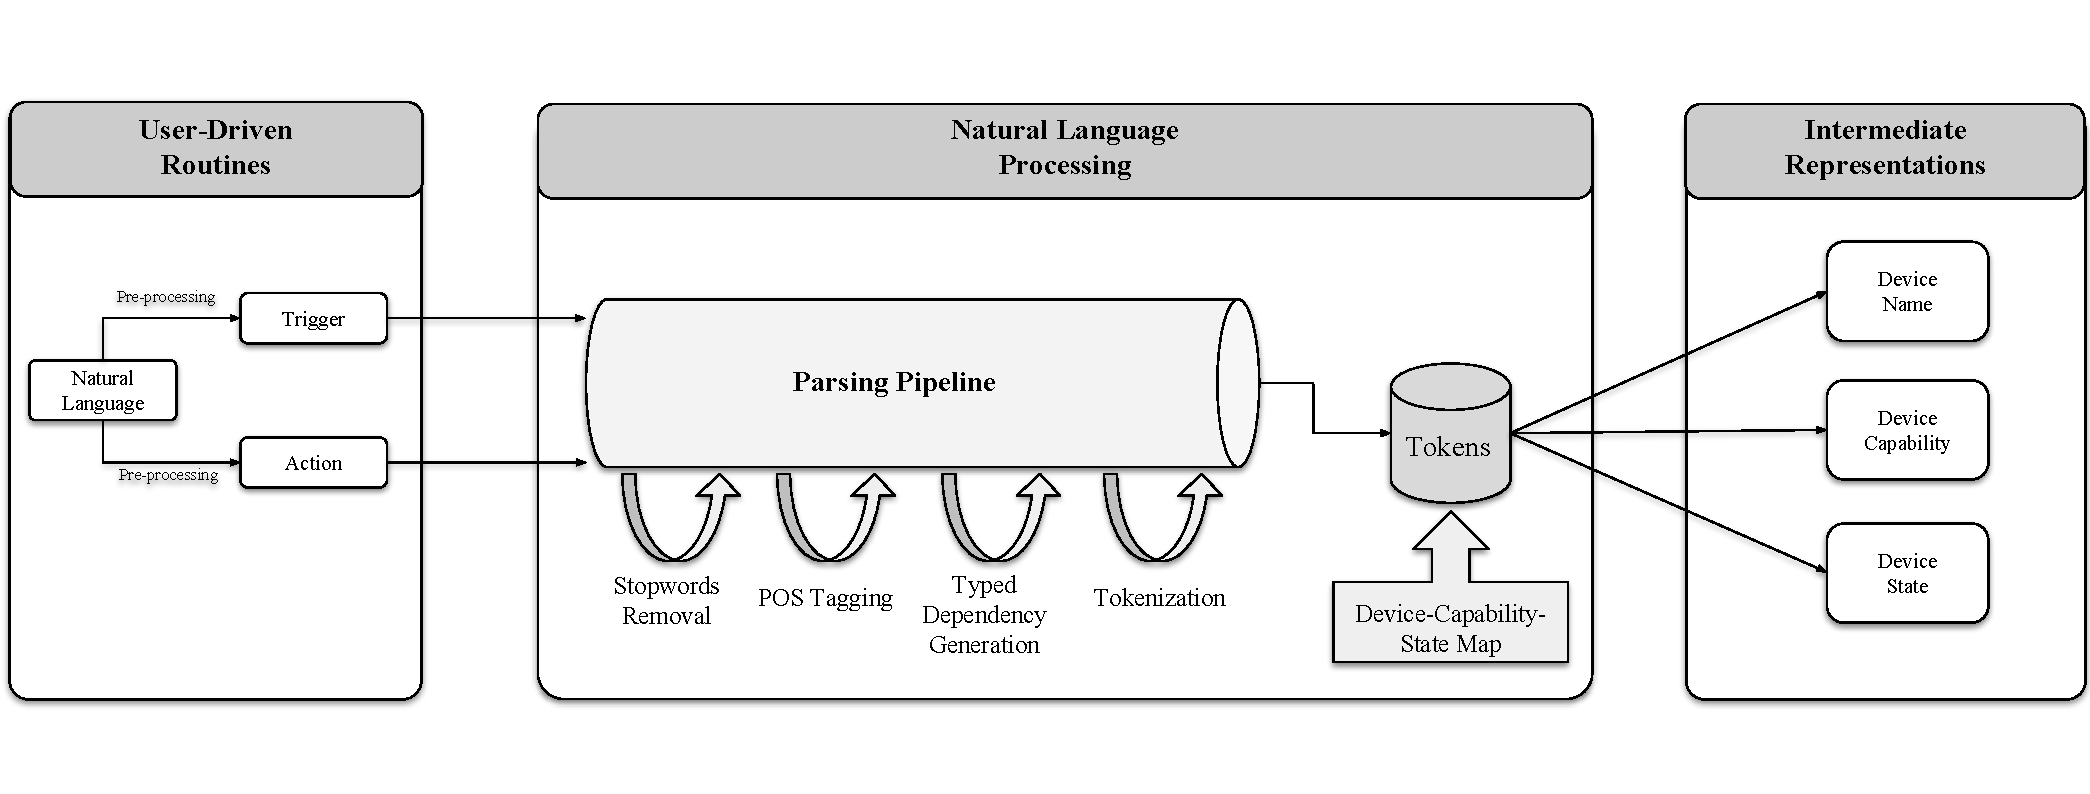
\includegraphics[width=\textwidth]{figs/nlp-tool-final.pdf}
    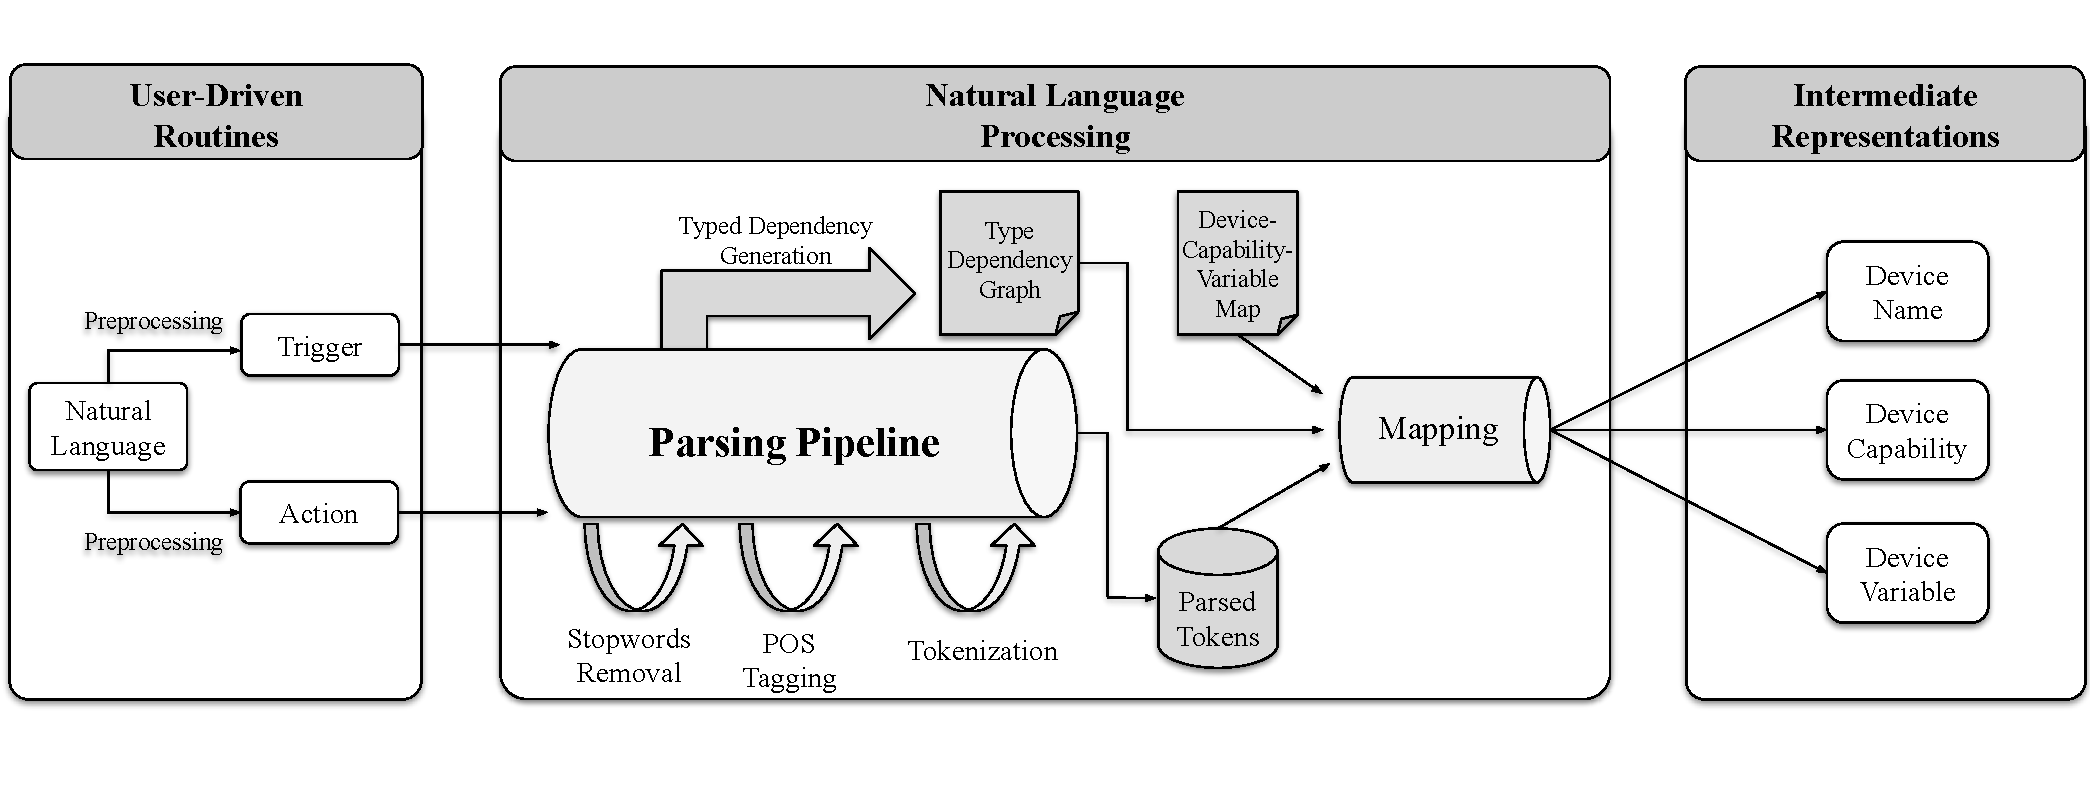
\includegraphics[width=\textwidth]{figs/nlp-tool-final-v2.pdf}
    \caption{Overview of the framework for transforming user-driven routines into intermediate representation (IR)}
    \label{fig:nlp-framework}
\end{figure*}




In this section, we will describe our design choices of our approach of transforming user-driven routine to intermediate representation. Figure.~\ref{fig:nlp-framework} provides an overview of the three main stages.


\subsection{Design choices}
One of the other main goals of this project is to be able to generate intermediate representation \textit{automatically}. In order to automate the process of converting user written routines to execution indicators for systematic testing, we use NLP techniques to extract devices information from human written routines. We extract and
correlate the behaviors in three layers: {\sf (1)} device name, {\sf (2)} device capability, and {\sf (3)} device variable (state).

As mentioned before, this approach consists of three main steps. In Step 1, we \textit{pre-processes} user-driven routines through splitting them by ``If'' and ``Then'', these syntactic indicators were provided for participants when creating routines. Since both the trigger and action should each contain all the device information needed to generate the intermediate representation, we could treat them as the same problem and pass them into the same program following the same procedure.

Although triggers and actions might seem to be distinct at first glance, they share sufficient amount of similarity that can be consider equivalent in terms of being considered as input to our models (one for each intermediate representation type).

We can list the similarities as the follows:
\begin{itemize}
    \item \textbf{Similarity 1:} Triggers and actions both have to specify the three characteristics of the devices in one way or another. For example: If air temperature is greater than 80, turn on the air conditioner. Both trigger and action have to specify some characteristic about the device.
    \item \textbf{Similarity 2:} Trigger are often expressed as an action, and the reverse is also true. For example, ``turn on the light'' can act both as the trigger of one routine and as the action of another. This demonstrates that there is not much difference in the essence of the phrase.
\end{itemize}
% Proof that trigger and action are the same

One other design decision we made is that we required participants of the survey to use conjunction ``AND'' or ``OR'' in all capitalized characters when combining the different trigger conditions. This is to help our models to recognize each distinct trigger condition more accurately without imposing much constraint on user. 

Some triggers, such as Location Mode and Time, does not have a physical device associated with them. In those cases, we create a new device type called ``Null'' with the respective capabilities to incorporate them. By doing so, we were able to prevent ourselves to omit some virtual trigger conditions.

Following the pre-processing procedure in the above manner, we can obtain a list of triggers conditions and a list of actions. For the proof of concept, we implement this approach on the list of triggers. Applying this method to the list of actions is trivial, all we have to do is to replace the input from trigger conditions to the action phrases.

The processed triggers will then be pass into the next stage, the Parsing Pipeline, where the major part of the Natural Language Processing takes place. After trying out different part of speech taggers, we settled with Stanford CoreNLP POS Tagger~\cite{Manning2014} as it was able to perform better than the default NLTK POS Tagger.

The result of the Parsing Pipeline, combine with the addition of the device-capability-variable map and type dependency graph, will then be mapped into the resulting three intermediate representation.



\subsection{Preprocessor}

Our pre-processor accepts plain English text as the input and reduces the number of lexical tokens by eliminating unnecessary words and unrecognizable characters or words. In particular, the preprocessor performs the following pre-processing tasks:
\begin{itemize}
    \item \textbf{Comparison Handling: } Many routines contain value comparisons as their trigger conditions. However, since there is no constraint to what user can input, we observed that a substantial number of participants uses comparison operators (\eg ``>'', ``<'', etc) to construct their routines. Therefore, in order to have NLP tools to recognize these important symbols, We replaces all instances of comparison operators into English plain text. 
    \item \textbf{Stop words removal: } We follow standard NLP practices to pre-process our data, such as removing stop words (\eg ``a'', ``this'', ``the'') using NLTK library. 
    \item \textbf{Whitelisting input: } Since there is no enforcement in our user input, we whitelisted the routines using regular expression filtering. We only accepted a narrow set of input such as characters and numbers, and punctuation symbols as these sentences would become our input to the NLP parser.
\end{itemize}


\subsection{NLP Parser}
Our NLP Parser accepts the pre-processed sentences and annotates each words within a sentence using standard NLP techniques. We perform the following tasks with the Stanford CoreNLP parser:
\begin{itemize}
    \item \textbf{Name Entity Recognition: } We use the parser to identify named entities (\eg person names, organizations) in each routine. In addition, these entities are added to a dictionary so that we can perform additional natural language processing.
    \item \textbf{Part of Speech Tagging: }  We use Stanford POS Tagger to process each word in a given routine. We see that often the case that nouns are more related to the device name than the others; for example, ``smoke'' is good indicator of a ``smoke detector''.  While most cases are more complex than this example, we used this as one of our indicator for selecting the possible candidate for intermediate representation of Device Name. Similar approach can be used on identifying possible words that represents the Device Variables such as ``on'' or ``off'', which corresponds to part of speech ``IN'', preposition/subordinating conjunction. As for device capability, we noticed that they are generally associated with ``VB'', verb (\eg lock the door), would be mapped to door.lock.
    \item \textbf{Typed Dependency Generation: } Our more comprehensive analysis follows. Specifically, we use Stanford parser to annotate each routine with Stanford-typed dependency. One sample typed dependency graph generation of trigger condition is shown by Figure.~\ref{fig:dep-tree}. These information can be used later to help generating the intermediate representation mapping.
    \item \textbf{Tokenization: } When performing the above techniques, Stanford Parser would automatically tokenize each word in the sentence and output them as a tuple. This is important during the mapping phase since it saves the result of POS and type dependency generation with the associated word.
\end{itemize}

\subsection{Intermediate Representation Mapping}

From the result of the Parsing Pipeline, we were able to get a list of parsed tokens with valuable syntactic information associated with them. In order to create the three different types of intermediate representation, we would need to perform the mapping in three distinct ways. Before making different models, we created a device-capability-variable mapping with the all the devices mapped with its capabilities and with the possible variables / states that it can take. This mapping was done separately from the user-driven routines since it does not require any information from end-users. In order to create a model that can generate the desired intermediate representation, we would look at each token in a given routine, and examine its part of speech in addition to its typed dependency, and finally check for the device-capability-variable map as a way of confirmation.


\begin{figure}[t]
    %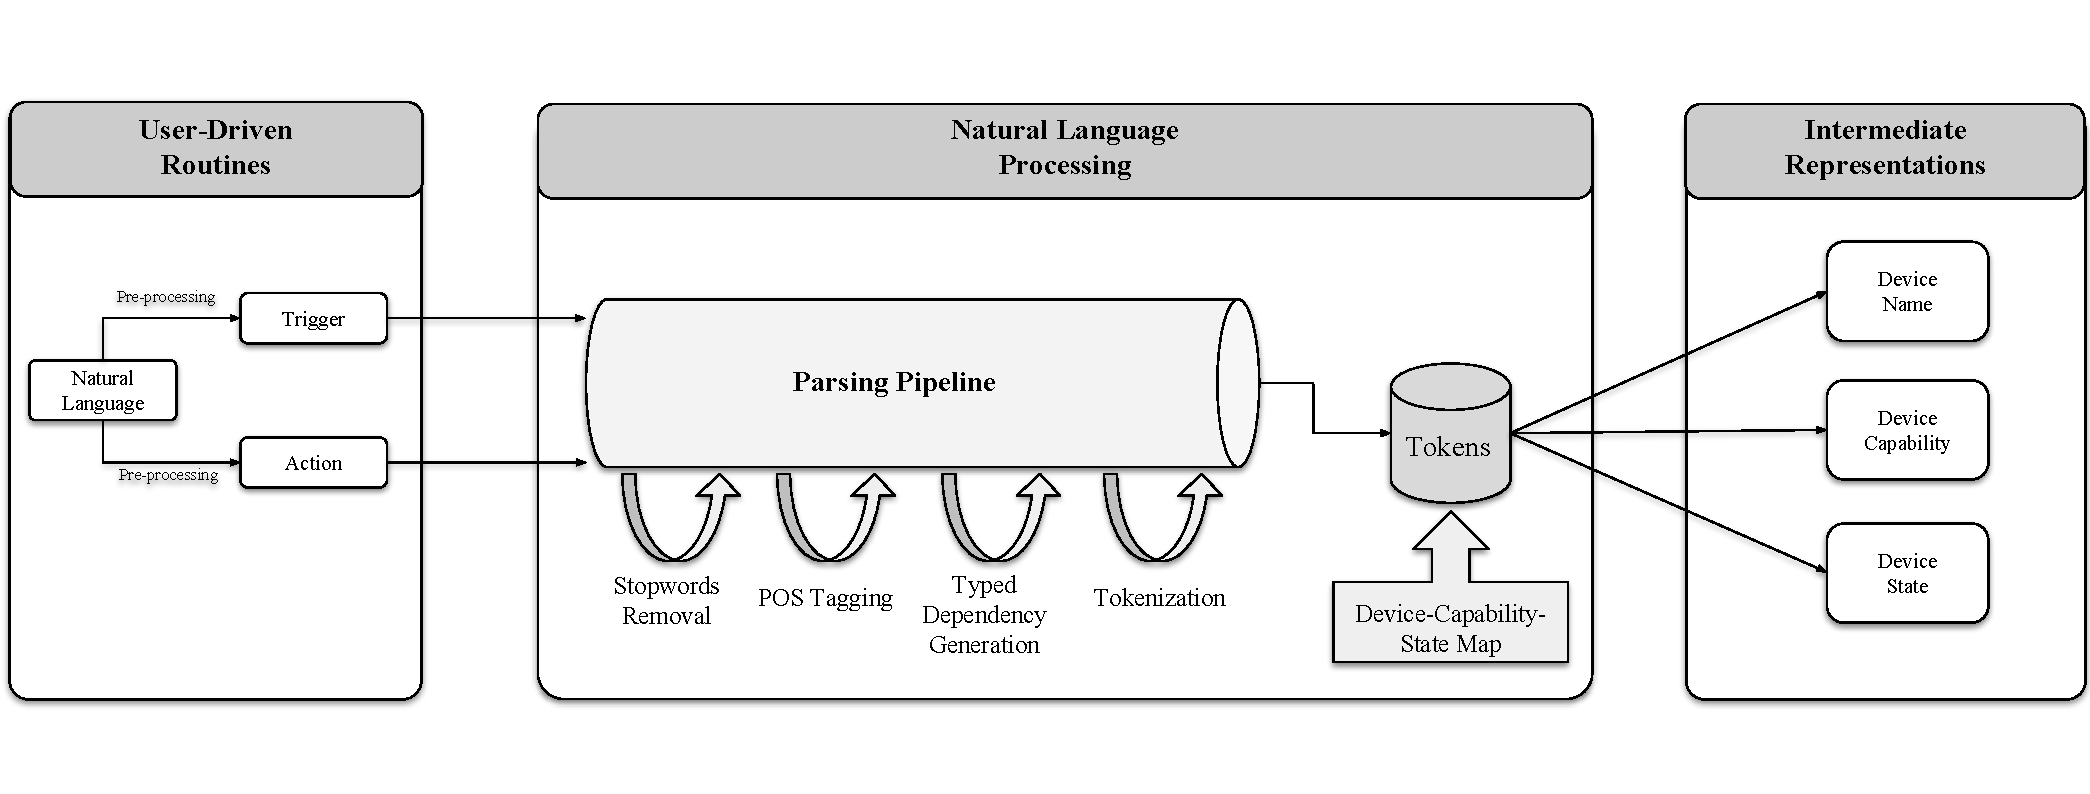
\includegraphics[width=\textwidth]{figs/nlp-tool-final.pdf}
    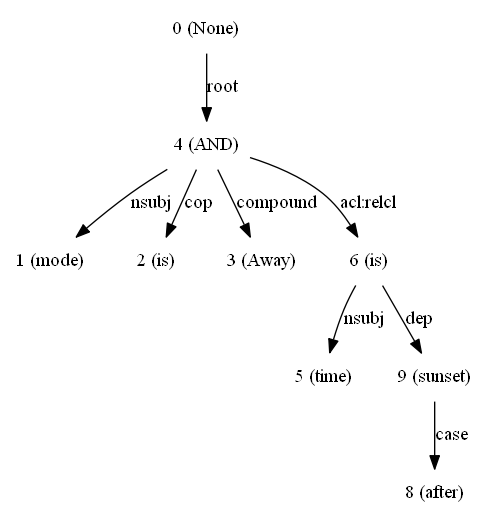
\includegraphics[width=3.5in]{figs/dep_good.png}
    \caption{Typed Dependency Graph of a Sample User-Driven Trigger}
    \label{fig:dep-tree}
\end{figure}




